% kuleuventheme2 by Janez Kren, September 2017, janez.kren@kuleuven.be, based on:
% kuleuventheme 1.3 by Roland Pastorino, 2013 roland.pastorino@kuleuven.be / www.rolandpastorino.com

\documentclass[11pt,t]{beamer}
\usetheme[sedes]{kuleuven2}	%THEME OPTIONS for LOGO: kul (default), kulak, lrd,    ; OPTIONS for TITLE PAGE: normal (default), sedes


%%% OTHER SETTINGS
\usefonttheme[onlymath]{serif}			% math font with serifs, delete to make it sans-serif
\setbeamertemplate{footline}[body] 		% delete this line to remove footline bar on all frames
%\usepackage[orientation=landscape,size=custom,width=16,height=9,scale=0.5,debug]{beamerposter} %enable for widescreen 16:9 ratio
%\titlegraphic{ \includegraphics[width=.2\paperwidth]{mytitlepagepic.png} } %optional title page image


%%% ADDED PACKAGES:
\usepackage[english]{babel}
\usepackage{amsfonts}
\usepackage{amssymb}

% Daniel packages
\usepackage{anyfontsize} % allowing font sizes at arbitrary sizes
\usepackage{amsbsy} % bold greek symbols in math mode
\usepackage{amsmath} % New line in math mode
\usepackage{pifont} % To add checkmark symbol

%%% TITLE PAGE INFO:
\title[Extending Idefix package]{Extending Idefix package} %[]] will appear in footline
\subtitle{Intermediate presentation}

\author{Daniel Gil Sanchez}
\institute{KU Leuven}
\date{March 2019}




\begin{document}
\csname beamer@calculateheadfoot\endcsname %recalculate head and foot dimension


 %%
 %%  0. TITLE PAGE and TABLE OF CONTENT
 %%
% Title page
\begin{frame}[plain,noframenumbering]
	\titlepage
\end{frame}
	

% Table of Contents
\begin{frame}{Outline}
	\hfill	{\large \parbox{.961\textwidth}{\tableofcontents[hideothersubsections]}}
\end{frame}

\section{Introduction}
\begin{frame}[fragile]{What is \textit{idefix} R package for?}
	\begin{itemize}
		\item To create optimal designs for discrete choice experiments (DCEs) based on the multinomial logit model (MNL) and
		\item Individually adapted designs for the mixed multinomial logit model (MIXL).
		\item Available on CRAN (v 0.3.3).
	\end{itemize}	
%	\pause	
	\begin{block}{Discrete choice experiments}
		DCEs are composed by:
		\begin{itemize}
			\item Nominal or Ordinal response variable
			\item Choice sets 
			\item Alternatives within each choice set
			\item Attributes and levels
		\end{itemize}
	\end{block}
\end{frame}

\begin{frame}[fragile]{Multinomial Logit Model}
	\begin{itemize}
		\item Choice design matrix $\mathbf{X} = [\mathbf{x}^{'}_{js}]$, where $\mathbf{x}_{js}$ is a $k \times 1$ vector of attributes for profile $j$ in choice set $s$.
		\item Respondent's utility is $u_{js} = \mathbf{x}^{'}_{js} \pmb{\beta}+ \epsilon_{js}$, where $\pmb{\beta}$ is a vector of parameters and $\epsilon_{js}$ is an i.i.d. extreme value error term.
		\item Probability a respondent chooses alternative $j$ in choice set $s$ is \\
			\vspace*{-4mm}
			$$p_{js}=\frac{e^{\mathbf{x}^{'}_{js} \beta}}{\sum^{J}_{t=1} e^{\mathbf{x}^{'}_{ts} \beta}}$$
		\item Information Matrix is \\ 
		\vspace*{-5mm}
			$$\mathbf{M}(\mathbf{X},\pmb{\beta}) = N \sum_{s=1}^{S} \mathbf{X}^{'}_s(\mathbf{P}_s-\mathbf{p}_s\mathbf{p}_s^{'})\mathbf{X}_s$$
			where $\mathbf{X}_s$ is the design matrix of choice set $s$, $\mathbf{p}_s = [p_{1s},\cdots,p_{Js}]$ and $\mathbf{P}_s = diag[p_{1s},\cdots,p_{Js}]$ and $N$ is the number of respondents.
	\end{itemize}
\end{frame}

\begin{frame}[fragile]{Optimality criteria}
	\begin{itemize}
		\item To obtain precise estimates of $\pmb{\beta}$
		\begin{itemize}
			\item \textcolor{kul-blue}{$\mathit{D}-$optimality: minimize the determinant of the variance-covariance matrix of $\pmb{\beta}$}
			\item $\mathit{A}-$optimality: minimize the trace of the variance-covariance matrix of $\pmb{\beta}$
		\end{itemize}
		\item To obtain precise response predictions
		\begin{itemize}
			\item $\mathit{G}-$optimality: minimize the maximum prediction variance
			\item $\mathit{V}-$optimality: minimize the average prediction variance
		\end{itemize}					
	\end{itemize}
%	\pause
	\begin{alertblock}{Note:}
		These criteria are based on the information matrix, which depends on the unknown values in $\pmb{\beta}$ through the probabilities $p_{js}$. Therefore, a Bayesian strategy that integrates the design criteria over a prior parameter distribution $\pmb{\pi(\beta)}$ is adopted. Usually, the prior is a multivariate normal distribution.
	\end{alertblock}
\end{frame}

\begin{frame}[fragile]{D-optimality}
	\begin{itemize}
		\item In OLS is defined as $D = |\mathbf{X}^{'}\mathbf{X}|$
		\item In MNL is defined adopting the prior distribution of $\pmb{\beta}$
		$$D_B = \int_{\mathcal{R}^k} \left\{det\left(\mathbf{M}^{-1}(\mathbf{X},\pmb{\beta}\right)\right\}^{1/k}\pi(\pmb{\beta})d\pmb{\beta}$$

Where $k$ is the number of unknown parameters in the model and $\pi(\pmb{\beta})$ is the prior distribution of $\pmb{\beta}$. This criterion is also called Bayesian $D-$optimality criterion or just $D_B$.
	\end{itemize}
\end{frame}

\begin{frame}[fragile]{Mixed Multinomial Logit model}
	\begin{itemize}
		\item MNL models assume that the respondents have the same preferences, $\pmb{\beta}$, for the attributes studied in the experiment.
		\item MIXL models assume that the individual preferences, $\pmb{\beta}_n$, follow a certain distribution across respondents ($\pmb{\beta}_n \sim f(\pmb{\mu}_\beta,\pmb{\sigma}_\beta)$).
		\begin{itemize}
			\item Probability a respondent chooses alternative $j$ in choice set $s$ is \\
			\vspace*{-3mm}
			$$p^{*}_{js}=\int p_{js}(\pmb{\beta})f(\pmb{\beta}) d\beta $$
			Where $p_{js}(\pmb{\beta})$ is defined as in the MNL model.
		\end{itemize}
	\end{itemize}
	\begin{block}{}
	MIXL model assumes that respondents choose according to an MNL model, but each with different preferences.
	\end{block}
\end{frame}

\begin{frame}[fragile]{Individually Adapted designs}
The proper name of the methodology is \textit{Individually adapted sequential Bayesian} design. It consists in two stages:
	\begin{itemize}
		\item \textbf{Initial static stage:} use a common initial prior distribution $\pmb{\pi}(\beta)$ for all respondents. It is used to generate an initial design.
		\item \textbf{Adaptative sequential stage:} the prior information  is updated sequentially after each response, and each choice set is constructed using the updated prior. Therefore, each respondent will have a different design.
	\end{itemize}
	\begin{alertblock}{Notes:}
	\begin{itemize}
		\item Any criterion can be used to select a new choice set.
		\item Different algorithms can be used to select a new choice set. Here the Modified Fedorov Algorithm is used.
	\end{itemize}
	\end{alertblock}
\end{frame}

\begin{frame}[fragile]{Current state of the package}
\begin{figure}
			\centering
			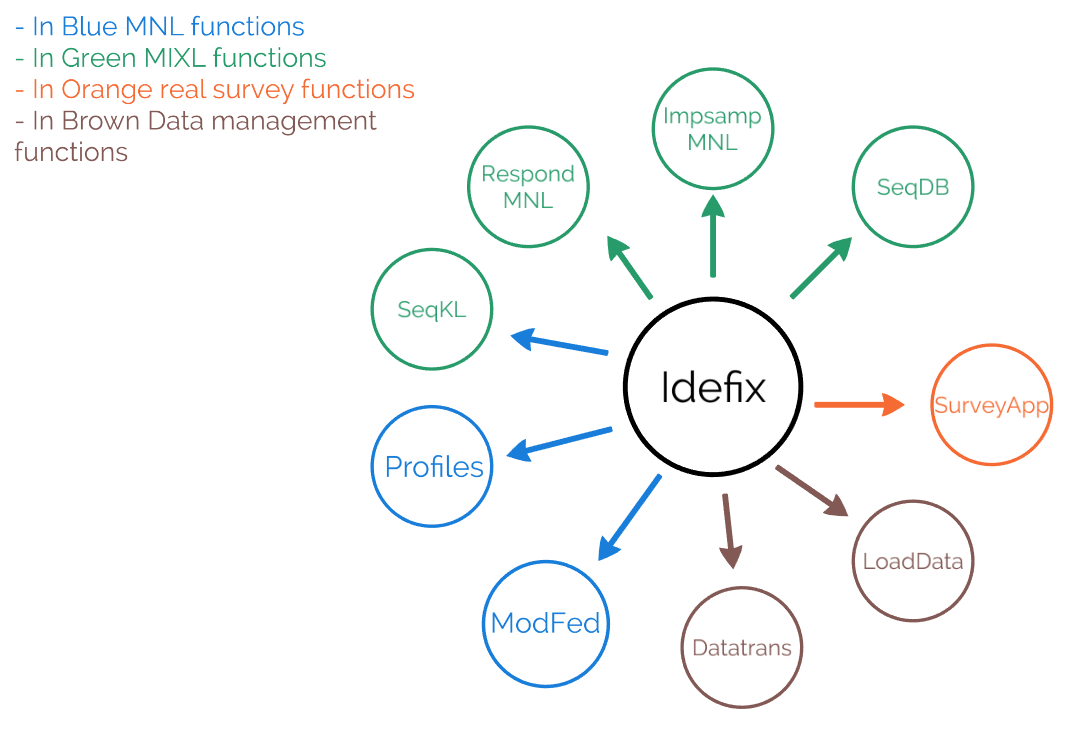
\includegraphics[scale = .5]{mygraphics/CurrentState.png}
		%\caption{Example graphic \label{fig:figure1}}
		\end{figure}
\end{frame}

\begin{frame}[fragile]{Objectives}
	\begin{enumerate}
		\item Improve processing time of the \textbf{Modified Fedorov algorithm} by implementing some parts of the algorithm in C++. %\pause
		\item Implement the \textbf{KL criterion} and compare it with the function that is already available in the package.
		\item Implement the \textbf{Coordinate Exchange algorithm} to create optimal designs.
		\item Make a \textbf{simulation study} to compare processing times and optimality of designs between the Modified Fedorov algorithm, the Coordinate Exchange algorithm and the use of DB and KL criteria.
		\item Reorganize some functions inside the package, remove possible redundancy in code and implement parts of the code in C++.
	\end{enumerate}
\end{frame}

\section{Modified Fedorov Algorithm}
%Difference between Fedorov and Modified Fedorov
%https://documentation.sas.com/?docsetId=qcug&docsetTarget=qcug_optex_details33.htm&docsetVersion=14.2&locale=en
\begin{frame}{Modified Fedorov Algorithm}
	\begin{itemize}
		\item Point exchange algorithm
		\item Algorithm steps:
		\begin{enumerate}
			\item Create a random initial design from candidate set.
			\item For each row of this design
			\begin{enumerate}
				\item Exchange this row with each row from the candidate set. Resulting in N different designs.
				\item Compute optimality criterion for each modified design and choose the best value.
				\item update initial design and start again with the following row
			\end{enumerate}
			\item Repeat this process until no differences are found between the initial design and the final.
		\end{enumerate}
	\end{itemize}
\end{frame}

\begin{frame}[fragile]{Modified Fedorov Algorithm}
\textbf{Example}\\
\begin{itemize}
	\item Design $3^3/2/8$ $\Rightarrow$ Design matrix $16 \times 6$ (dummy coding).
	\item Candidate set has $3^3 = 27$ rows/profiles
	\item In each iteration $16 \times 27 = 432$ information matrices and determinants are computed to find the best optimal design. Assume that only one iteration is needed.
	\item But, the information matrix needs draws from the prior of $\beta$. Assuming just 10 draws, the number of information matrices and determinants is $4320$.
	\item But, different random initial designs to avoid local optima. Assuming 10 initial designs, the final number of information matrices and determinants is $43200$.
\end{itemize}	
\end{frame}

\begin{frame}[fragile]{Processing time}
\textbf{First activity: Improve processing time in individually adapted designs.}\\
	\texttt{SeqDB} function selects the next DB-efficient choice set given parameter values and an initial design.
	
	\begin{exampleblock}{Example}
		Considering $3^3/2/8$ design:
		\begin{figure}
			\centering
			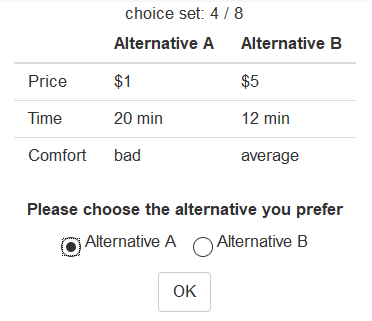
\includegraphics[scale = .5]{mygraphics/choiceset.png}
		%\caption{Example graphic \label{fig:figure1}}
		\end{figure}
	\end{exampleblock}
\end{frame}

\begin{frame}[fragile]{Processing time}
	\textbf{How to make it faster?}\\
	Using Hadley Wickham approach in his book \textit{Advanced R}:
	\begin{enumerate}
		\item Find the biggest bottleneck (the slowest part of the code).
		\item Try to eliminate it (you may not succeed but that is ok).
		\item Repeat until your code is \textbf{fast enough}.
	\end{enumerate}
	
	\begin{block}{But, how to make it faster?}
	\begin{itemize}
		\item Using faster functions in R and avoiding loops using vectorized functions.
		\item Implementing parts of the code in C++.
	\end{itemize}		
	\end{block}
\end{frame}

\begin{frame}[fragile]{Processing time}
	\textbf{Find the biggest bottleneck}
	\begin{itemize}
		\item $4 \times 3 \times 2/2/8$ design.
		\item 10 draws from $\beta$ distribution.
		\item Pre-defined initial design and alternatives chosen (1st stage of IASB approach).
	\end{itemize}
\end{frame}

\begin{frame}[fragile]{Processing time}
\textbf{Profiling \texttt{SeqDB} function}
\begin{figure}
			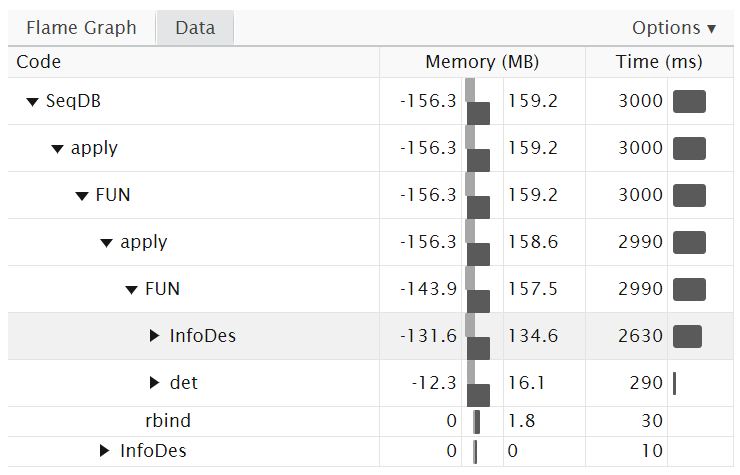
\includegraphics[scale = .7]{mygraphics/Profiling1.png}
		%\caption{Example graphic \label{fig:figure1}}
		\end{figure}
\end{frame}

\begin{frame}[fragile]{Processing time}
\textbf{Implementation in C++}
\begin{itemize}
	\item Use of Rcpp package
	\item Use of Rcpp Armadillo: C++ linear algebra library
\end{itemize}
\vspace*{-3mm}
	\pause
	\begin{center}~
	% box2 = light gray background and kul-blue text
		\begin{beamercolorbox}[wd=.85\textwidth,sep=4pt,center]{box2}	
		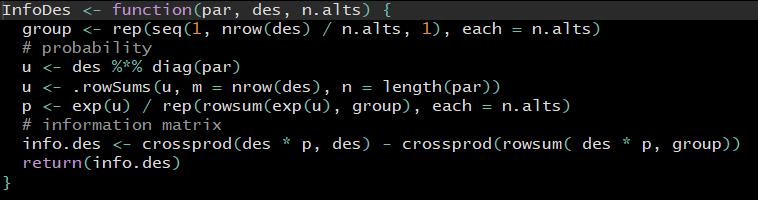
\includegraphics[scale = .7]{mygraphics/Code1.png}
		\end{beamercolorbox}
		\hspace{2pt}
		\begin{beamercolorbox}[wd=.1\textwidth,sep=4pt,center]{box2}	
		 10 lines \\ of code
		\end{beamercolorbox}
	\end{center}
	\vspace*{-7mm}
	\pause
	\begin{center}~
	% box2 = light gray background and kul-blue text
		\begin{beamercolorbox}[wd=.85\textwidth,sep=4pt,center]{box2}	
		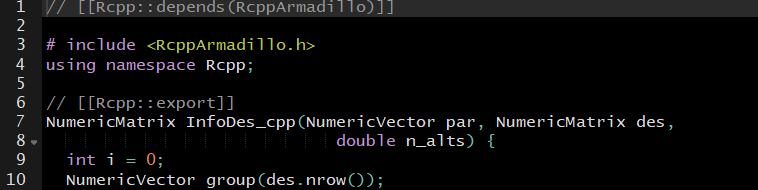
\includegraphics[scale = .7]{mygraphics/Code2.png}
		\end{beamercolorbox}
		\hspace{2pt}
		\begin{beamercolorbox}[wd=.1\textwidth,sep=4pt,center]{box2}	
		 117 lines \\ of code
		\end{beamercolorbox}
	\end{center}
\end{frame}

\begin{frame}[fragile]{Processing time}
\textbf{Result:} Implementation in C++ is almost 6x faster.
	\vspace*{-3mm}
	\begin{center}
		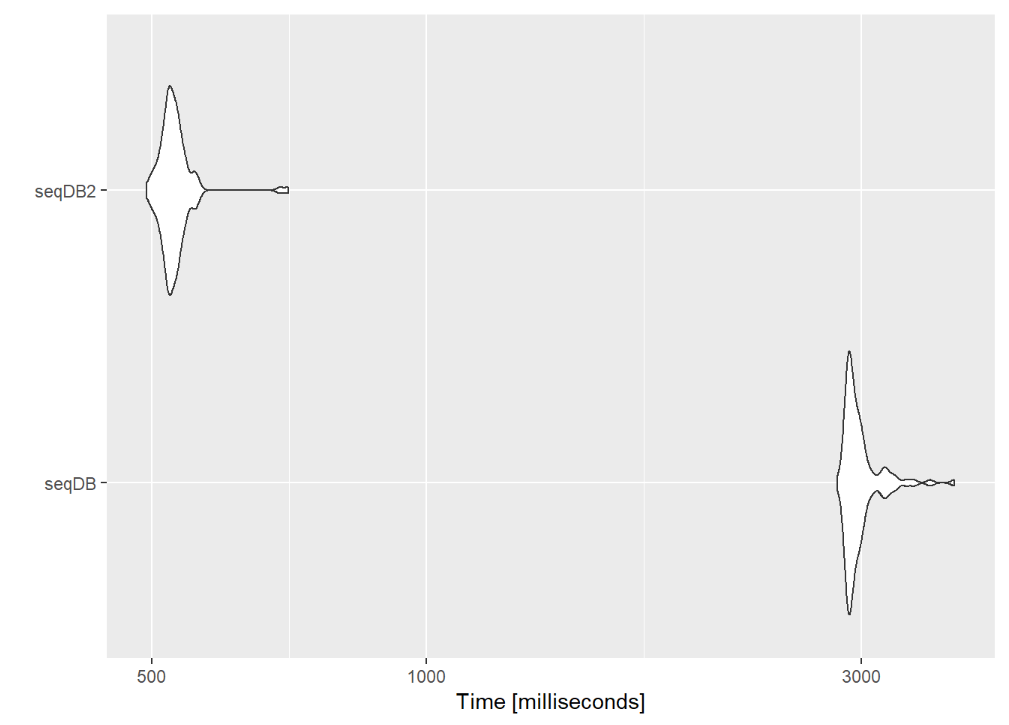
\includegraphics[scale = .5]{mygraphics/benchmark1.png}
	\end{center}
\end{frame}

\begin{frame}[fragile]{Processing time}
	Find next bottleneck and improve it (multiple times)
	\vspace*{-3mm}
	\begin{center}
		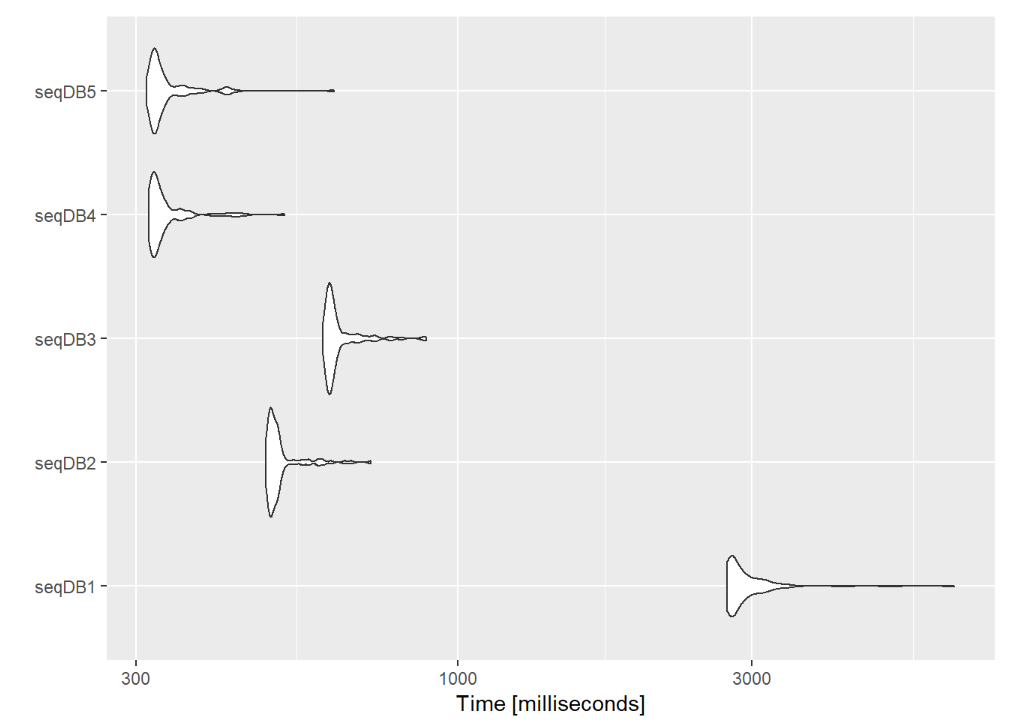
\includegraphics[scale = .5]{mygraphics/benchmark2.png}
	\end{center}
\end{frame}

\begin{frame}[fragile]{Processing time}
	What about parallel computing?
	\vspace*{-3mm}
	\begin{center}
		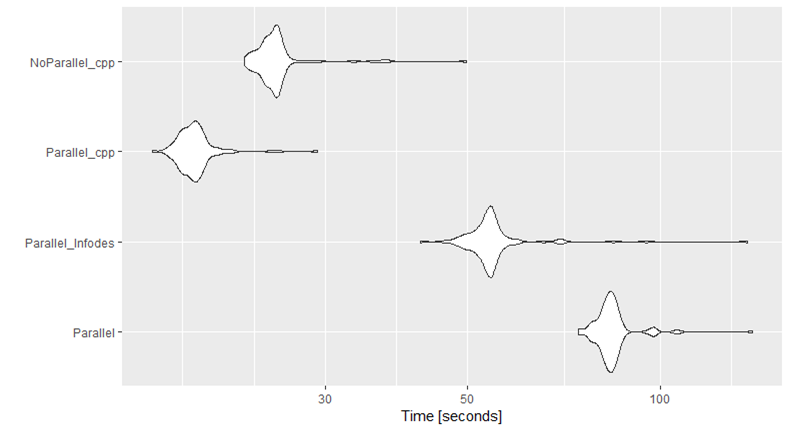
\includegraphics[scale = .4]{mygraphics/benchmark3.png}
	\end{center}
\end{frame}

\begin{frame}[fragile]{Processing time}
	\textbf{Second activity: Improve processing time in MNL designs}	
	\begin{itemize}
		\item The hardest work had already been done
		\begin{itemize}
			\item Find bottlenecks
			\item Improve functions in C++
		\end{itemize}
		\item \texttt{ModFed} processing time was also improved by using the same functions as in \texttt{SeqDB}.
	\end{itemize}
	\pause
	\begin{block}{What was needed to complete this task with success?}
		\begin{itemize}
			\item Understand how Modified Fedorov algorithm works.
			\item Learn version control (Git and GitHub).
			\item Learn how C++ and C++ armadillo work in R.
			\item Learn about benchmarking and parallel computing.
		\end{itemize}
	\end{block}
\end{frame}

%%%%%%%%%%%%%%%%%%%%%%%%%%%%%%%%%%%%%%%%%%%%%%%%%%%%

\section{Kullback-Leibler criterion}

\begin{frame}[fragile]{Kullback-Leibler criterion}
	\begin{itemize}
		\item It was developed under individually adapted designs for the MIXL.
		\item It is an alternative to $D-$optimal criterion.
		\item It is faster to compute and it provides equally efficient designs.
		\item It is based on the Kullback-Leibler information:
		$$KL(f,g) = \int f(x) log \frac{f(x)}{g(x)}dx$$
		Where f and g are continuous densities of $X$.
		\begin{itemize}
			\item $KL$ is non-negative or zero ($f(x)=g(x)$)
			\item $KL$ increases as the densities become more divergent
			\item $KL$ is not symmetric, $KL(f,g) \neq KL(g,f)$
		\end{itemize}
	\end{itemize}
\end{frame}

\begin{frame}[fragile]{Kullback-Leibler criterion}
\textbf{Implementation in DCEs}
\begin{itemize}
	\item To select next choice set, maximize the $KL$ between the current posterior of $\beta$ and the updated posterior one can obtain with the additional response from the next choice set.
	\item Since there are multiple alternatives, the expectation over all possible choices is maximized.
	\vspace*{-2mm}
	$$KLP = \sum_{j=1}^J \pi (y_{jsn}|\mathbf{y}_n^{s-1}) KL\left[f(\pmb{\beta})_n|\mathbf{y}_n^{s-1}), f(\pmb{\beta})_n|\mathbf{y}_n^{s-1},y_{jsn})\right]$$
	Where $s$ is the next choice set, $n$ is a particular respondent and $j$ is the chosen alternative. The densities $f(\pmb{\beta})_n|\mathbf{y}_n^{s-1})$ and $f(\pmb{\beta})_n|\mathbf{y}_n^{s-1},y_{jsn})$ are the updated posteriors and $\pi (y_{jsn}|\mathbf{y}_n^{s-1})$ is the posterior weighted choice probabilities for the alternatives in the choice set $s$, given the previous responses.
\end{itemize}
\end{frame}

\begin{frame}[fragile]{Kullback-Leibler criterion}
	\textbf{Implementation in the package}
	\begin{itemize}
		\item Applying $KL$ definition, $KLP$ can be written as
$$KLP = \sum_{j=1}^J \pi (y_{jsn}|\mathbf{y}_n^{s-1}) [ log \ \pi (y_{jsn}|\mathbf{y}_n^{s-1}) - $$ \\ $$\int log \ p_{jsn}(\pmb{\beta}_n)f(\pmb{\beta}_n|\mathbf{y}_n^{s-1} d \pmb{\beta}_n) ]$$

		\item Modified Fedorov algorithm is used, but instead of using $D-$optimality criterion $KLP$ is used.
		%\item In theory it should be faster because no information matrix nor determinant is computed but only posterior weighted choice probabilities.
		\item Simulations in R are not consistent with results obtained in the paper that proposed the criterion.
	\end{itemize}
\end{frame}

\begin{frame}[fragile]{Kullback-Leibler criterion}
	\textbf{Third activity: Check why \textit{SeqKL} function is not working}
	\begin{itemize}
		\item Check code of simulations done in the paper that proposed the criterion.
		\begin{itemize}
			\item Made in SAS. Proc IML.
			\item $490$ lines of code. No comments, no indentation.
		\end{itemize}
		\item Check code of implementation in R
		\item Comparison of results from each function in both implementations.
		\item List differences.
		\item Discussion.

	\end{itemize}
\end{frame}

\section{Coordinate Exchange Algorithm}
\begin{frame}[fragile]{Coordinate Exchange Algorithm}
\begin{itemize}
	\item Coordinate exchange algorithm
	\begin{itemize}
		\item Point exchange algorithm: Compute optimality criterion $\prod_{j=1}^J l_j$ times for each row.
		\item Here: Compute optimality criterion $\sum_{j=1}^J l_j$ times for each row.
	\end{itemize}
	\item Algorithm steps:
	\begin{enumerate}
		\item Create a random initial design
		\item For each row of this design
		\begin{enumerate}
			\item Take the first attribute in the row, evaluate the optimality criterion over all the levels of that attribute.
			\item If the optimality criterion of any of these levels is better than the current, then it is replaced.
			\item Repeat with the remaining attributes in the row.
		\end{enumerate}
		\item Repeat this process until no differences are found between the initial design and the final.
	\end{enumerate}
\end{itemize}
\end{frame}

\begin{frame}[fragile]{Coordinate Exchange Algorithm}
\textbf{Example}\\
\begin{itemize}
	\item Design $3^3/2/8$ $\Rightarrow$ Design matrix $16 \times 6$ (dummy coding).
	\item No Candidate set is needed.
	\item In each iteration $16 \times 9 = 144$ information matrices and determinants are computed to find the best optimal design. Assume that only one iteration is needed.
	\item But, the information matrix needs draws from the prior of $\beta$. Assuming just 10 draws, the number of information matrices and determinants is $1440$.
	\item But, different random initial designs to avoid local optima. Assuming 10 initial designs, the final number of information matrices and determinants is $14400$.
\end{itemize}	
\small{\textit{As a reminder, in Modified Fedorov the final number was $43200$.}}
\end{frame}

\begin{frame}[fragile]{Coordinate Exchange Algorithm}
\textbf{Fourth activity: Implement the Coordinate Exchange algorithm}
\begin{enumerate}
	\item \textcolor{kul-blue}{Implementation with only categorical factors/attributes.}
	\item Implementation with continuous attributes.
	\item Implementation with both categorical and continuous.
	\item Improve processing time, if possible (parallel computing, C++).
\end{enumerate}
\begin{alertblock}{Note:}
	$D-$optimality criterion is going to be used, so the implementation of the information matrix in C++ is also going to be used here.
\end{alertblock}
\end{frame}

\section{Simulation study}
\begin{frame}[fragile]{Simulation study}
	\begin{itemize}
		\item The idea is to compare the processing time of Modified Fedorov algorithm and the Coordinate Exchange algorithm.
		\begin{itemize}
			\item Determine the scenarios where one outperforms the other.
			\item Determine in which situations parallel computing is needed.
		\end{itemize}
		\item Compare efficiency of designs found with $D-$optimality criterion and $KL$ criterion.
		\begin{itemize}
			\item Determine the scenarios where one outperforms the other.
		\end{itemize}
	\end{itemize}
\end{frame}

\begin{frame}[fragile]{Objectives}
	\begin{enumerate}
		\item Improve processing time of the \textbf{Modified Fedorov algorithm} by implementing some parts of the algorithm in C++. \textcolor{red}{\checkmark} %\pause
		\item Implement the \textbf{KL criterion} and compare it with the function that is already available in the package. \textcolor{red}{\checkmark} %\pause
		\item Implement the \textbf{Coordinate Exchange algorithm} to create optimal designs. %\pause
		\item Make a \textbf{simulation study} to compare processing times and optimality of designs between the Modified Fedorov algorithm, the Coordinate Exchange algorithm and the use of DB and KL criteria. %\pause
		\item Reorganize some functions inside the package, remove possible redundancy in code and implement parts of the code in C++. \textcolor{red}{\checkmark}
	\end{enumerate}
\end{frame}

\begin{frame}[c,plain,noframenumbering]
\begin{tikzpicture}[remember picture,overlay]
\fill[fill=black]
    (current page.south east)  rectangle  (current page.north west)   ;
\end{tikzpicture}

\centering
%\textcolor{white}{\textit{Statistics is the grammar of science}}\\
%\raggedleft	\normalfont \textcolor{white}{Karl Pearson}
\end{frame}

%\appendix
%\begin{frame}[noframenumbering,label=extraframe]{Extra slide}
%
%Because of frame option [noframenumbering] this frame is not counted in the total number of frames.
%
%\vspace{24pt}
%This button with cross-referencing link that will take you back to the frame: 
%
%\hyperlink{buttons}{\beamerreturnbutton{Back to Buttons}}
%\end{frame}

\end{document}
